\documentclass[12pt]{article}
\usepackage[utf8]{inputenc}
\usepackage{amsmath}
\usepackage{amsfonts}
\usepackage{amsthm}
\usepackage{array}
\usepackage{graphicx}
\usepackage{parskip}
\usepackage{fancyhdr}
\usepackage{tikz}
\usepackage{float}
\usepackage{listings}
\usepackage{color}
\usepackage{caption}
\usepackage{longtable}
\usepackage[nottoc]{tocbibind}
\usepackage[cache=false,section]{minted}
\usepackage[a4paper, total={6in, 8in}]{geometry}
\usepackage[ruled]{algorithm2e}
\usepackage{glossaries}
\usemintedstyle{default}
\newminted{haskell}{frame=lines,framerule=2pt}
\newminted{R}{frame=lines,framerule=2pt}
\graphicspath{{./images/}}

\tikzstyle{bag} = [align=center]

\makeglossaries

\newacronym{dp}{DP}{Dynamic Pipeline Paradigm}
\newacronym{bfs}{BFS}{Breadth-First Search}
\newacronym{dfs}{DFS}{Depth-First Search}
\newacronym{wcc}{WCC}{Weak Connected Components}
\newacronym{haskell}{Haskell}{Haskell Programming Language}
\newacronym{fp}{FP}{Functional Programming}
\newacronym{rl}{R}{R Language}

\title{Towards a Haskell Abstraction of Dynamic Pipeline Paradigm}
\author{
\begin{tabular}{c c}       
      \normalsize{Juan Pablo Royo Sales} & \normalsize{Edelmira Pasarella}\\ 
      \footnotesize{Universitat Politècnica de Catalunya} & \footnotesize{Computer Science Department}\\
      \footnotesize{Barcelona - Spain} & \footnotesize{Universitat Politècnica de Catalunya}\\ 
      \footnotesize{\texttt{juan.pablo.royo@estudiantat.upc.edu}} & \footnotesize{Barcelona - Spain}\\ 
      \footnotesize{} & \footnotesize{\texttt{edelmira@cs.upc.edu}}\\\\
      \normalsize{Cristina Zoltan} & \normalsize{Maria-Esther Vidal}\\ 
      \footnotesize{Computer Science Department} & \footnotesize{TIB Leibniz Information Center for Science and Technology and}\\
      \footnotesize{Universitat Politècnica de Catalunya} & \footnotesize{L3S Research Cneter, Hannover, Germany}\\ 
      \footnotesize{Barcelona - Spain} & \footnotesize{\texttt{maria.vidal@tib.eu}}\\ 
      \footnotesize{\texttt{zoltan@cs.upc.edu}} & \footnotesize{}\\ 
\end{tabular}
}

\pagestyle{fancy}
\fancyhf{}
\fancyhead[L]{Dynamic Pipeline on Haskell}
\fancyhead[R]{\thepage}
\fancyfoot[L,C]{}
\setlength{\headheight}{15pt}
\renewcommand{\headrulewidth}{0pt}
\renewcommand{\footrulewidth}{0pt}
\newtheorem{hyp}{Hypothesis}
\date{}

\begin{document}

\maketitle
\begin{abstract}
\textit{Dynamic Pipeline Paradigm} has been defined in order to solve problems where the data is heterogeneous 
and in motion. Taking advantage on pipelining stage parallelization, this paradigm allows to dynamically adapt 
stage computations according to the input. It has been shown in the definition of this computational model that any
implementation attempt of the Paradigm requires fast and flexible parallelization techniques as well as tools that 
are suitable with the notion of Computation as a First Class Citizen. In this work we implement \textit{Dynamic Pipeline Paradigm}
using \texttt{Haskell} for \textit{Finding Connected Components of a Graph} as a primary example problem. We show different results 
and how \texttt{Haskell} behaves on that context showing that it is a suitable Language for implementing \textit{Dynamic Pipeline Paradigm} 
not only because its strong theoretical foundations which provides a strong manipulations of Computations as primary entities, but also because it has a powerful 
Set of Tools for writing multithreading and parallel computations with optimal performance.
\end{abstract}

\section{Introduction}
\textit{\acrfull{dp}} has been defined in~\cite{dp_def} along side with some examples problems that are suitable to be solved with this Computational Model.
One of those problems is \textit{Finding Connected Components of an Undirected Graph}, which is known as a \textbf{\acrfull{wcc}} problem. 
Given an Undirected Graph $G = (V, E)$, we can find \acrshort{wcc} of $G$ in $O(V + E)$ using \textit{\acrfull{dfs}} or \textit{\acrfull{bfs}} algorithm~\cite{CormenLeisersonEtAl09}. 
Although this problem can be solved in linear complexity time, when we are manipulating real Graphs, which are usually big, it would be better to have a more suitable Computational Model where this can be done with
optimal performance. \acrshort{dp} with its \textit{Parallelization Pipeline model} improve that performance on Big Graphs for finding \acrshort{wcc}.
One of the biggest challenge of \acrshort{dp} is to find a proper Set of Tools and Language which can take advantage from both: Fast Parallel processing and Strong theoretical foundations that manage computations as First Class Citizens. 
On that sense we conduct with this work an implementation of \acrshort{dp} for solving \acrshort{wcc} with \acrfull{haskell} showing that both aspects are covered.

\textbf{Objective:} We show that \acrshort{haskell} it is a suitable Language for implementing \acrshort{dp} working with the problem of \acrshort{wcc}, in order to further create an Abstraction Library or Framework
to solve other Problems with \acrshort{dp} in \acrshort{haskell}.
In that sense we show the techniques and tools used on the language to achieve the desired goal as well as the measurements taken to empirically show how this solution behave in terms of performance and parallelization.

\textbf{Contributions:} We start to create and define an abstraction of \acrshort{dp} in \acrshort{haskell} which is going to allow use this new tool set for solving other computational problems that fits with this Computational Model.

\section{Connected Components of Graph using DP}
\textbf{Here we should put the Pseudo Code of DP Connected Components}

\section{DP for finding WCC on Haskell: Implementation}
In this section we are going to show all the implementation details for building a \acrshort{dp} Abstraction in \acrshort{haskell} solving \acrshort{wcc} problem.
There are two main components in \acrshort{dp} model which requires a careful choice to succeed in the implementation of the model: Parallelization to support Pipeline Parallel processing without penalizing global computation and Channels to link and communicate 
the different stages of the pipeline. We can argue that another special components is the dynamic generation of the computations or \textit{Filters}, but choosing a \acrfull{fp} Language like \acrshort{haskell} allow us to represent
that for free with \textit{Anamorphisms} and \textit{Catamorphisms}~\cite{lenses}.\footnote{All the Source Code of this work can be found here https://github.com/jproyo/upc-miri-tfm/tree/feature/library-v1/connected-comp}

\subsection{Parallelization}
One of the most important components on this implementation is the selection of \textbf{Concurrency Library} to support an intensive load on parallelism. A direct guess to achieve this
could be to use \textit{Monad Par} based on this work~\cite{monad_par}, but we have discarded that since we want to achieve Parallelism at Thread level and not to Spark level, due to the nature
of \acrshort{dp} where the approach of the model is Pipeline Parallelism and not Data Parallelism. The next obvious choice is to use \mintinline{haskell}{forkIO :: IO () -> IO ThreadId} from \mintinline{bash}{base}
module, but that would imply to handle all the threads lifecycle, terminations and errors in a custom manner. We choose \textbf{async}\footnote{https://hackage.haskell.org/package/async} 
library which allow us to spawn asynchronous computations~\cite{parallel_book} on \acrshort{haskell}.

\subsection{Channels}\label{section:channels}
The other important component in \acrshort{dp} model are \textit{Channels}. In this case we implement Channels using \textbf{unagi-chan}\footnote{https://hackage.haskell.org/package/unagi-chan} library which among other things
it has the following characteristics compare with other approaches:

\begin{itemize}
  \item \mintinline{haskell}{MVar} Channel with \textbf{no} use of \mintinline{haskell}{STM}: This allows to avoid internal locking for concurrent access. In this case
  we can use this advantage because in \acrshort{dp} model, one specific \textit{Pipeline Stage} which is running in a separated thread can only access to its \textit{Inputs/Outputs} channels for \textit{Reading/Writing} accordingly 
  and those operations are not concurrently share by other Threads (\textit{Stages}) for the same Channels.  
  \item \textbf{Non-Blocking} Channels: This library contains blocking and non-blocking Channels for reading and this is a key aspect to gain performance and speed up on the implementation.
  \item Optimized for $x86$ Architectures with use of low-level \textit{fetch-and-add} instructions.
  \item $100x$ faster on Benchmarking compare with \mintinline{haskell}{STM} and default base \mintinline{haskell}{Chan} implementations.
\end{itemize}

\subsection{Property Based Testing}
In order to test some properties of our implementation we use \textit{QuickCheck}~\cite{quickcheck} for the generation of Arbitrary Graphs with Arbitrary number of Connected Components, which are processed
by our algorithm later to prove that the same amount of \acrshort{wcc} are calculated as well.

\subsection{DP Connected Components Implementation}

\textbf{Principal Algorithm of DP:}
The following is the principal algorithm which represents the \textit{Monadic} computation of the principal \textit{Stages} that 
compose \acrshort{dp} model: \textit{Input, Generator and Output}. 

\begin{listing}[H]
\begin{minted}[fontsize=\small,numbers=left,frame=lines,framerule=2pt,framesep=2mm,baselinestretch=1.2,highlightlines={2,11}]{haskell}

runParallelDP :: Handle -> IO ()
runParallelDP h = input h >>= generator >>= output

input :: Handle -> IO (DP.Stream Edge ConnectedComponents)
input h = fromInput h >>= (|>> parseEdges)

output :: ConnCompDP -> IO ()
output = DP.mapM (R.putStrLn . show)

fromInput :: Handle -> IO (DP.Stream ByteString ConnectedComponents)
fromInput h = DP.unfoldM (B.hGetLine h) (R.hIsEOF h)

parseEdges :: ByteString -> IO [Edge]
parseEdges = toEdge . decodeUtf8

\end{minted}
\caption{Main algorithm \acrshort{dp} for \acrshort{wcc}}
\label{src:haskell:1}
\end{listing}

We can appreciate in the line 11~\ref{src:haskell:1} the use of the \mintinline{haskell}{unfoldM} which has been defined in the Abstraction \acrshort{haskell} Library.
It can be seen that the implementation of the problem in \acrshort{haskell} matches almost identically to the formal definition of \acrshort{dp} model.
It is important to notice that the input is being read in \textbf{non-blocking} mode and by batches of bytes allowing the streaming computation as long as the edges arrives to the 
\textit{Generator} or the first \textit{Filter} Stages\footnote{The format of the input file for the case of this example is a plain format where each line contains an Edge of the Graph in and both vertices are separated by a blank space.}.

\textbf{Generator:}
The \textit{Generator} is the Computation in the Pipeline which is responsible to know when to interpose a new \textit{Filter} in front of the Pipe.
In the case of \acrshort{wcc} a new \textit{Filter} is created on each new Edge that arrives to the \textit{Generator}.

\begin{listing}[H]
\begin{minted}[fontsize=\small,numbers=left,frame=lines,framerule=2pt,framesep=2mm,baselinestretch=1.2,highlightlines={2,11}]{haskell}
generator :: ConnCompDP -> IO ConnCompDP
generator = DP.foldrS createNewFilter
  where
    createNewFilter c v = do
      newInput  <- newChan
      newOutput <- newChan
      DP.Stream newInput newOutput 
            <$> async (newFilter (toConnectedComp v) c newInput newOutput)
  
  \end{minted}
  \caption{Generator \acrshort{dp} for \acrshort{wcc}}
  \label{src:haskell:2}
\end{listing}

As we can appreciate here, the highlighted line 2 shows the use of the \acrshort{haskell} Abstraction which is a \textit{Catamorphism} which at the same time is reducing the \textit{Stream}
it is creating the \textit{Stages} in the middle of the Pipe. We are going to describe later this \textbf{combinator}.

\textbf{Filters:}
In this case the algorithm is not as succinct as the previous because here is where the 2-step calculation takes place. As we have explained before each \textit{Filter} contains 2 sequential 
computations which are called \mintinline{haskell}{actor1} and \mintinline{haskell}{actor2}. The first one is responsible for gathering Connected Components based on the first Edge from wich 
this \textit{Filter} was created for, and the second \textit{Actor} is responsible for Union its own calculated Connected Components with others that are coming from the downstream.

\begin{listing}[H]
\begin{minted}[fontsize=\small,numbers=left,frame=lines,framerule=2pt,framesep=2mm,baselinestretch=1.2,highlightlines={16-20,33-36}]{haskell}
newFilter :: ConnectedComponents
          -> ConnCompDP
          -> DP.Channel Edge
          -> DP.Channel ConnectedComponents
          -> IO ()
newFilter conn inCh toInCh outCh = actor1 conn inCh toInCh >>= actor2 inCh toInCh outCh

actor1 :: ConnectedComponents 
       -> ConnCompDP 
      -> DP.Channel Edge
      -> IO ConnectedComponents
actor1 conn inCh toInCh = maybe finishActor doActor =<< DP.pullIn inCh
where
  finishActor = DP.end' toInCh >> return conn

  doActor v
    | v `includedIncident` conn = do
      let newList = v `addToConnectedComp` conn
      actor1 newList inCh toInCh
    | otherwise = v `DP.push'` toInCh >> actor1 conn inCh toInCh


actor2 :: ConnCompDP
      -> DP.Channel Edge 
      -> DP.Channel ConnectedComponents 
      -> ConnectedComponents
      -> IO ()
actor2 inCh toInCh outCh conn = maybe finishActor doActor =<< DP.pullOut inCh

where
  finishActor = conn `DP.push'` outCh >> DP.end' outCh

  doActor cc 
    | conn `intersect` cc = let newCC = conn `union` cc 
                             in actor2 inCh toInCh outCh newCC
    | otherwise           = cc `DP.push'` outCh >> actor2 inCh toInCh outCh conn
\end{minted}
\caption{Generator \acrshort{dp} for \acrshort{wcc}}
\label{src:haskell:3}
\end{listing}

As we can see here the, the algorithm for managing the Sets and do the \textit{Intersection} and \textit{Union} are not optimal\label{not:optimal}
\footnote{The propose of the present work is to present the implementation of \acrshort{dp} with \acrshort{haskell} but not working in the most optimal calculation of \acrshort{wcc}} and are base
on \mintinline{haskell}{Data.Set} module provided by \textbf{containers}\footnote{https://hackage.haskell.org/package/containers} library.

\section{DP Haskell Abstraction: An approximation}
This is a first approximation to a more robust library that we are working for building \acrshort{dp} Algorithms using \acrshort{haskell}
\footnote{This first version of the abstraction is under construction and it will probably differ by the time of the Conference presentation}.
As we have stated before~\ref{section:channels}, we use \mintinline{haskell}{Control.Concurrent.Chan.Unagi.NoBlocking} Channels. 
This is similar to the \textbf{Type} definition of channels that we can find here~\cite{parallel_book}, where the channels is a combination of an Input, where 
we can read-only and an Output where we can write only, avoiding as much as possible race conditions and concurrency issues.
On top of that we are defining a \mintinline{haskell}{Stream a b} Type which contains an Input \mintinline{haskell}{Channel a} and an Output \mintinline{haskell}{Channel b} 
plus a computation which process that streaming from Input to Output. That computation is a \mintinline{haskell}{process :: Async ()}.

\begin{listing}[H]
\begin{minted}[fontsize=\small,numbers=left,frame=lines,framerule=2pt,framesep=2mm,baselinestretch=1.2,highlightlines={}]{haskell}  
type Channel a = (InChan (Maybe a), OutChan (Maybe a))

data Stream a b = Stream
  { inChannel  :: Channel a
  , outChannel :: Channel b
  , process    :: Async ()
  }

\end{minted}
\caption{\acrshort{dp} \acrshort{haskell} Abstraction}
\label{src:haskell:4}
\end{listing}

We define several combinators that are helpful to manipulate those \mintinline{haskell}{Stream a b} types and build the \acrshort{dp}

\begin{table}[H]
  \begin{tabular}{|l|l|}
   \hline
   Function :: Type & Description\\
   \hline
   \mintinline{haskell}{endIn :: Stream a b -> IO ()} & Mark the EOF of the Input Channel \\
   \hline
   \mintinline{haskell}{endOut :: Stream a b -> IO ()} & Mark the EOF of the Output Channel \\
   \hline
   \mintinline{haskell}{pushOut :: b -> Stream a b -> IO ()} & Write value \mintinline{haskell}{b} into Output Channel \\
   \hline
   \mintinline{haskell}{pushIn :: a -> Stream a b -> IO ()} & Write value \mintinline{haskell}{a} into Input Channel \\
   \hline
   \mintinline{haskell}{pullIn :: Stream a b -> IO (Maybe b)} & Read possible value \mintinline{haskell}{b} from Output Channel \\
   \hline
   \mintinline{haskell}{pullOut :: Stream a b -> IO (Maybe a)} & Read possible value \mintinline{haskell}{a} from Input Channel \\
   \hline
  \end{tabular}
 \caption{Main combinators}
 \label{table:1}
 \end{table}
 
Apart from this combinators there are some specials one that requires more explanation because they are use on main \acrshort{dp} algorithm
like \mintinline{haskell}{foldrS} or \mintinline{haskell}{unfoldM}.

\begin{listing}[H]
\begin{minted}[fontsize=\small,numbers=left,frame=lines,framerule=2pt,framesep=2mm,baselinestretch=1.2,highlightlines={}]{haskell}    

{-# INLINE foldrS #-}
foldrS :: (Stream a b -> a -> IO (Stream a b)) -> Stream a b -> IO (Stream a b)
foldrS = loop
 where
  loop fio c = maybe (return c) (loop fio <=< fio c) =<< pullIn c

-- Generate Stream base on a seed function `f`
{-# INLINE unfoldM #-}
unfoldM :: IO a -> IO Bool -> IO (Stream a b)
unfoldM f stop = do
  newCh  <- newChan
  newCh' <- newChan
  end' newCh'
  Stream newCh newCh' <$> async (loop newCh)
  where loop newCh = ifM stop (end' newCh) (f >>= (`push'` newCh) >> loop newCh)

{-# INLINE mapM #-}
mapM :: (b -> IO c) -> Stream a b -> IO ()
mapM f inCh = async loop >>= wait
  where loop = maybe (pure ()) (\a -> f a >> loop) =<< pullOut inCh

{-# INLINE foldMap #-}
foldMap :: Monoid m => (b -> m) -> Stream a b -> IO m
foldMap m s = async (loop mempty) >>= wait
  where loop xs = maybe (pure xs) (loop . mappend xs . m) =<< pullOut s

\end{minted}
\caption{\acrshort{dp} \acrshort{haskell} Abstraction}
\label{src:haskell:5}
\end{listing}

It can be seen the powerful expressiveness of \acrshort{haskell} Language that we can define \mintinline{haskell}{foldrS} in one line. This combinator
allow us to generate on demand new filters as long as the values are arriving to the generator, which is known as a \textit{Catamorphism}.

In the case of \mintinline{haskell}{unfoldM} which is its counterpart, an \textit{Anamorphism}, it is a little more complex because a \mintinline{haskell}{Stream a b} 
requires an \mintinline{haskell}{Async ()} computation as a part of the structure and we need to generate that as long as our seed function do not stop with \mintinline{haskell}{IO Bool} computation.

\mintinline{haskell}{mapM} and \mintinline{haskell}{foldMap} are specialization for \mintinline{haskell}{Stream a b} where \mintinline{haskell}{pullOut} is used for mapping or folding
the consumer part of the \textit{Stream}.

\section{Experiments and Discussion}
In this work we have conducted $2$ kind of experiments in order to test our assumptions and verify the correctness of the implementation.

\begin{itemize}
  \item \textbf{Automated Testing}: This was conducted under Test Unit Library \textit{hspec}\footnote{https://hackage.haskell.org/package/hspec} alongside \textit{QuickCheck} as we mentioned
  before to generate Random Graphs and put under different set of Connected components auto-generated graph the algorithm.
  \item \textbf{Real Graph Analysis}: In this case we have selected some Graphs from \textbf{Stanford Network Data Set Collection}\footnote{https://snap.stanford.edu/data/index.html} and analyze how the implementation
  behaves under bigger and real Graphs.
  \item \textbf{Performance Analysis}: Regarding performance analysis we have gather profiling data from \textit{GHC} for one of the Real Graph, in order to measure how the program performs on Multithreading execution and 
  on Memory Allocation.
\end{itemize}

\subsection{Automated Testing and QuickCheck}
\textbf{Automated Cases:} Regarding the automated cases, we have defined 6 small examples with the following particularities to be automated and be tested automatically on every run of \textit{hspec}. In that sense
we are sure that every modification to the principal algorithm, improve of the code or refactor are verified against this cases for free. 

\begin{table}[H]
  \centering
  \begin{tabular}{|l|l|l|}
   \hline
   Graph case & Edges & Ordered (Edges)\\
   \hline
   1 \acrshort{wcc} & 5 & YES \\
   \hline
   1 \acrshort{wcc} & 5 & NO \\
   \hline
   2 \acrshort{wcc} & 8 & YES \\
   \hline
   1 \acrshort{wcc} & 6 & YES \\
   \hline
   3 \acrshort{wcc} & 11 & YES \\
   \hline
   3 \acrshort{wcc} & 11 & NO \\
   \hline
  \end{tabular}
 \caption{Test Cases}
 \label{table:2}
 \end{table}

\begin{listing}[H]
\begin{minted}[fontsize=\small,numbers=left,frame=lines,framerule=2pt,framesep=2mm,baselinestretch=1.2,highlightlines={}]{haskell}      
it "Example 3 CC - Shuffle" $ do
  let input = "1 2\n 2 3\n 4 5\n 1 4\n 1 3\n 7 8\n 10 12\n 3 5\n 3 6\n 7 9\n 11 10\n"
  result <- liftIO $ runParallelWithExample input
  length result `shouldBe` 3
\end{minted}
\caption{Example \textit{hspec} Testing}
\label{src:haskell:6}
\end{listing}

\textbf{QuickCheck:} In this case the main challenge consist on how to write \mintinline{haskell}{Arbitrary} derivations, in order to 
allow \textit{QuickCheck} to generate a Graph $G$ and at the same time control the amount of Connected Components that we want for $G$, 
in order to verify the following property: Given a Graph $G$, $cc : G \to \mathbb{N}$ is the Function that gets the Number of Connected Components of $G$.
Then,

\begin{equation}
  \forall G, cc(G) = DP(G)
\end{equation}

In our QuickCheck derivation this is the following:

\begin{listing}[H]
  \begin{minted}[fontsize=\small,numbers=left,frame=lines,framerule=2pt,framesep=2mm,baselinestretch=1.2,highlightlines={}]{haskell}      
newtype Edge a = Edge (a, a)
    deriving (Show, Eq, Ord)
  
newtype Graph = Graph { _gEdges :: Set (Edge Integer) } deriving (Show)
  
instance Arbitrary (Edge Integer) where
  arbitrary = do
    v1 <- getPositive <$> arbitrary
    v2 <- (getPositive <$> arbitrary) `suchThat` (/= v1)
    return $ Edge (v1, v2)
  
arbitraryGraphs :: Gen (Graph, Int)
arbitraryGraphs = do
  amount <- choose (1, 10)
  (, amount) <$> genGraph amount
  
genGraph :: Int -> Gen Graph
genGraph = fmap Graph . genConnComp
\end{minted}
\caption{QuickCheck \acrshort{dp}}
\label{src:haskell:7}
\end{listing}

We have avoid the details of \mintinline{haskell}{genConnComp} generator function, but it basically build a Set of Edges 
in which the amount of connected components should be the amount provided by parameter, which is randomly generated by QuickCheck.
Once we have QuickCheck generator we just need to tell QuickCheck how many examples we want to test to verify our property.

\begin{listing}[H]
\begin{minted}[fontsize=\small,numbers=left,frame=lines,framerule=2pt,framesep=2mm,baselinestretch=1.2,highlightlines={}]{haskell}      
context "Property Based Testing Examples"
  $ modifyMaxSuccess (const 1000)
  $ it "Retrieves the correct number of connected components"
  $ property
  $ forAll arbitraryGraphs 
  $ \(Graph{..}, amount) -> do 
    result <- liftIO $ runParallelWithExample $ toEdgesText _gEdges
    length result `shouldBe` amount
\end{minted}
\caption{QuickCheck Property Verification of \acrshort{dp}}
\label{src:haskell:8}
\end{listing}

\subsection{Real Graph Analysis}
As we have stated in the introduction of this section we have run our implementation against the following Stanford Networks:

\begin{table}[H]
  \centering
  \begin{tabular}{|l|l|l|l|}
   \hline
   \textbf{Network} & \textbf{Nodes} & \textbf{Edges} & \textbf{Nodes in the largest \acrshort{wcc}}\\
   \hline
   \text{Enron Emails~\cite{net_enron}} & 36692 & 183831 & 33696 \\
   \hline
   \text{Astro Physics Collaboration Net~\cite{net_astro}} & 18772 & 198110 & 17903 \\
   \hline
   \text{Google Web Graph~\cite{net_web_google}} & 875713 & 5105039 & 855802 \\
   \hline
  \end{tabular}
 \caption{Real Graph Analyzed}
 \label{table:4}
 \end{table}

\textbf{Results:} The following represents the execution for running these graphs on our \acrshort{dp} implementation.
\begin{table}[H]
  \centering
  \begin{tabular}{|l|l|l|l|l|}
   \hline
   \textbf{Network} & \textbf{Exec Param} & \textbf{MUT Time} & \textbf{GC Time} & \textbf{Total Time}\\
   \hline
   Enron Emails & \mintinline{bash}{+RTS -N4 -s} & 2.797s & 0.942s & 3.746s \\
   \hline
   Astro Physics Coll Net & \mintinline{bash}{+RTS -N4 -s} & 2.607s & 1.392s & 4.014s \\
   \hline
   Google Web Graph & \mintinline{bash}{+RTS -N8 -s} & 137.127s & 218.913s & 356.058s \\
   \hline
  \end{tabular}
 \caption{Execution times}
 \label{table:5}
 \end{table}

As we can see in~\ref{table:5} we are obtaining remarkable execution times even with the \textit{web-Google} Graph where we need to process $5$ Millions of Edges.
In order to compare better those times we have conducted a similar analysis on \acrfull{rl} using \textit{igraph} library.

\begin{listing}[H]
\begin{minted}[fontsize=\small,numbers=left,frame=lines,framerule=2pt,framesep=2mm,baselinestretch=1.2,highlightlines={6}]{r}      
> start_time <- Sys.time()
> g_ca <- read_graph("../data/ca-AstroPh.txt", format=c("edgelist"))
> length(decompose(g_ca, mode = c("weak")))
> end_time <- Sys.time()
> end_time - start_time
Time difference of 8.037778 secs
\end{minted}
\caption{R Language execution to measure time of \acrshort{wcc}}
\label{src:rlang:1}
\end{listing}

\begin{table}[H]
  \centering
  \begin{tabular}{|l|l|l|l|l|}
   \hline
   \textbf{Network} & \textbf{Total Time}\\
   \hline
   Enron Emails & 7.978754s \\
   \hline
   Astro Physics Coll Net & 8.037778s \\
   \hline
   \textbf{\textcolor{red}{Google Web Graph}} & \textbf{\textcolor{red}{51.2935s}} \\
   \hline
  \end{tabular}
 \caption{Execution time in R Language}
 \label{table:6}
 \end{table}

As we can appreciate on line 6~\ref{src:rlang:1} the amount of time taken by \acrshort{rl} in the case of \textit{AstroPh} collaboration network was $8.03$ seconds against
our solution which took only $4.014$ seconds. 
Although this repeats for several graphs bellow $500000$ edges, it is not the case with the \textit{web-Google} graph that has $5$ Million Edges which in our case took almost $6$ minutes, 
but in the case of \acrshort{rl} it took $52$ seconds. We have analyzed that case and as we have stated previously~\ref{not:optimal} our algorithm for the Second Actor where all the Connected Components are 
reduce, it is not optimal because it is out of the scope of this experiment to prove better complexity on Subgraph calculation.

\subsection{Performance Analysis}
For this type of analysis our experiment focus on \textit{email-Enron} Network only because profiling data generated by \textit{GHC} as any other profiling tool penalize execution time. 
On that sense we believe that the following data extracted from that experiment is quite enough to conclude how the implementation behave for the rest of the experiments.

\textbf{Multithreading:} For analyzing parallelization and multithreading we have used \textit{ThreadScope}\footnote{https://wiki.haskell.org/ThreadScope} which allows us to see how the parallelization is taking place
on \textit{GHC} at a fine grained level. In the following images we are going to see how this is behaving.

\begin{minipage}[t]{\linewidth}
  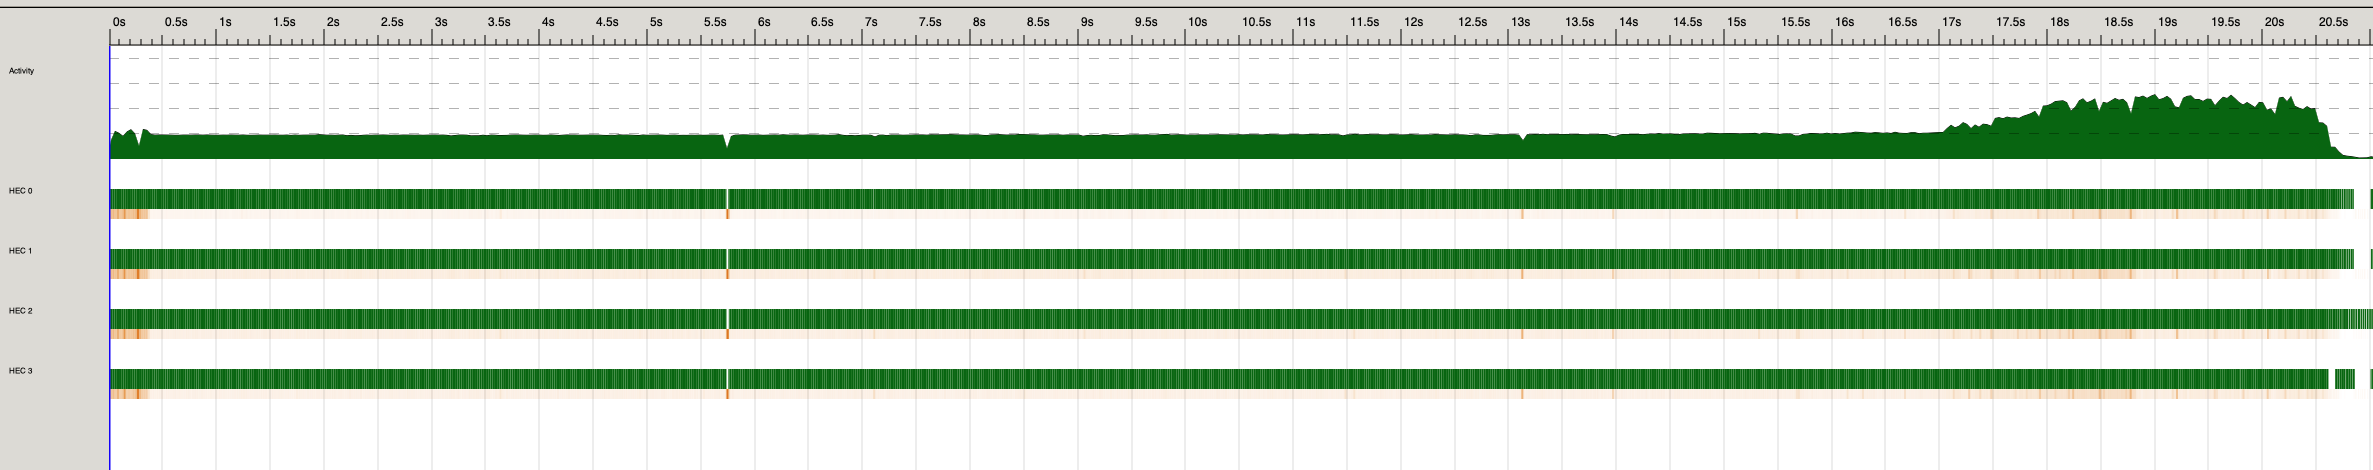
\includegraphics[width=\textwidth]{screen_1}
  \captionsetup{type=figure}
  \captionof{figure}{Threadscope Image of General Execution}
  \label{fig:1}
\end{minipage}

In this image we can see that the parallelization is being distributed evenly among the 4 Cores that we have set for this execution.
The distribution of the load is more intensive at the end of the execution where the Second phase of the algorithm is taking place and different filters are reaching execution of second Actor.
Although we are executing one of the selected real examples, the amount of work is not so significant for \textit{GHC} and the threads and distribution of the work keeps between 1 or 2 cores throughout 
the majority of the processing time.


\begin{minipage}[t]{\linewidth}
  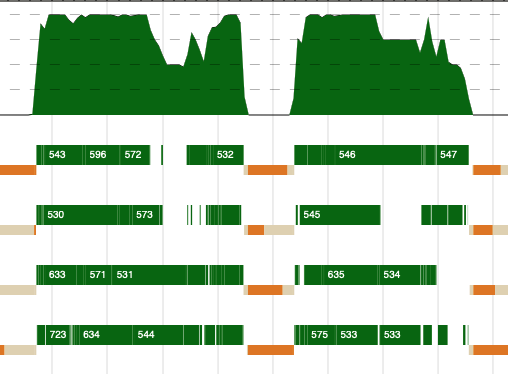
\includegraphics[width=\textwidth]{screen_2}
  \captionsetup{type=figure}
  \captionof{figure}{Threadscope Image of Zoomed Fraction}
  \label{fig:2}
\end{minipage}

In this second image, the numbers represents the number of \textit{Threads} that are being executed on that particular core.
We can verify again, in a much more detailed and and specific moment of the execution, our first assumption that the load is evenly distributed because the number of executing threads stay between $550$ and $600$
in average.

\textbf{Memory allocation:} Another important aspect in our case is how the memory is being handle to avoid Memory Leaks or other non-desired behavior, because our algorithm in particular \acrshort{wcc} requires
to maintain \textit{Connected Components} in memory throughout the execution of the program. 
In order to verify that our program does not have this problem, we measure memory allocation with \textit{eventlog2html}\footnote{https://mpickering.github.io/eventlog2html/} which converts generated profiling memory \mintinline{bash}{eventlog}
files into Graphical HTML representation. 

\begin{minipage}[t]{\linewidth}
  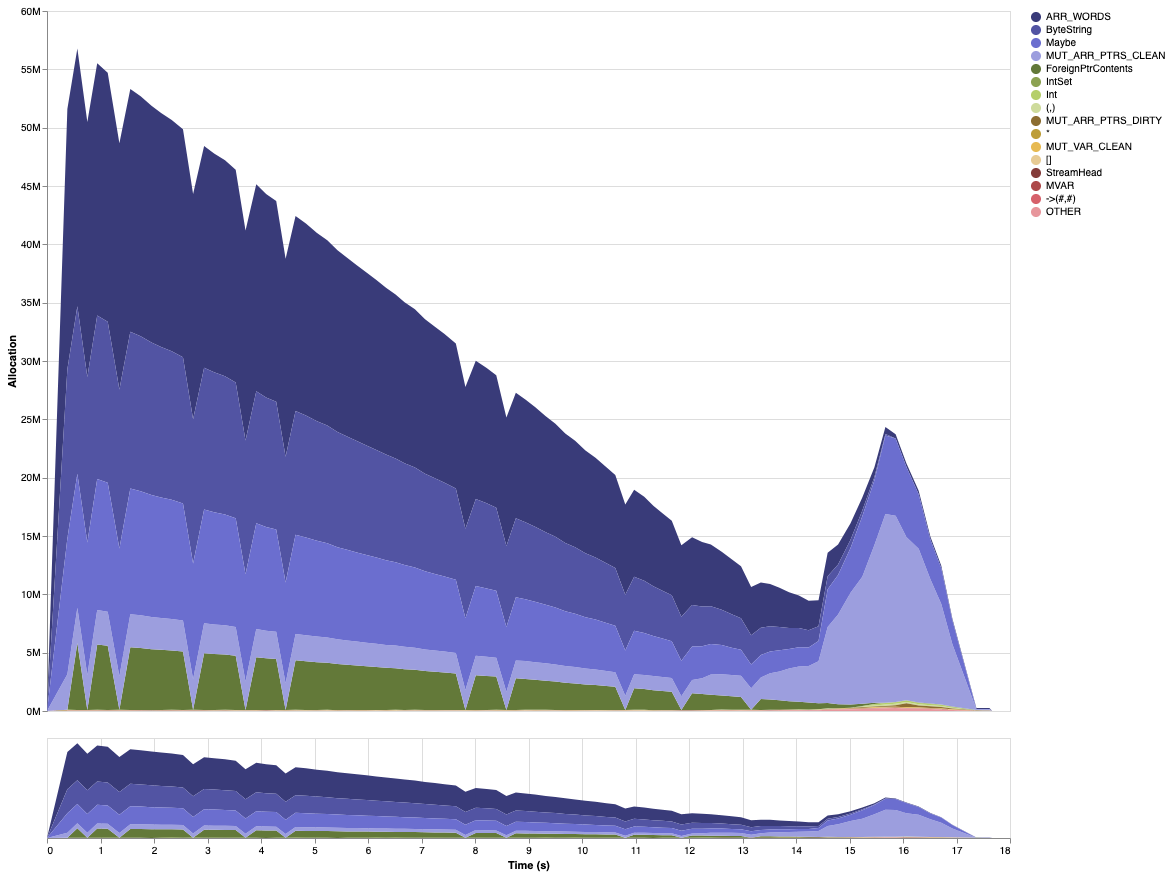
\includegraphics[width=\textwidth]{visualization}
  \captionsetup{type=figure}
  \captionof{figure}{Memory Allocation}
  \label{fig:3}
\end{minipage}

Regarding memory allocation we can see that our program does an optimal job on allocating memory since we are not using more than $60$ MB of memory.
Regarding how the memory is allocated during the execution of the program we can also appreciate that the memory is allocated at the beginning of the execution and steadily decrease over time.
The explanation for this is quite straightforward because at the beginning we are building all the filters and gathering the connected components (\textbf{Actor 1}). Once these \textit{Actors 1}
finish \textbf{Actor 2} start the execution shrinking Connected Components in Maximal connected components, releasing memory as it is being shown by profiler.
It is important to point out that this behavior is going to be present as long as the amount of the connected components is much more less than the amount of edges. If that is not the case this Graphical
representation will show a more linear Memory occupancy and not decreasing until the end of the program. 

\section{Future Work}
The aim of this work was to show that \acrshort{haskell} is a suitable and Strong Language to implement \acrfull{dp}. The explorations and experiments have shown that although 
the proposed solution behaves accordingly to what we have conceived, a better Abstraction and Description of the Paradigm should be done using all the mechanisms that the Language provides 
to allow future users of the library describe different algorithm in a straightforward manner.

Some of the aspects that needs to be addressed on the Abstraction are related to \textbf{Type Level Programming} techniques to ensure properties and proof on compilation time and use
of succinct combinators to allow different Effectful computations and not only restricted to \mintinline{haskell}{IO}. On the other hand a better definition of the \textit{Catamorphism} and \textit{Anamorphism}
combinators to use already provided abstraction for that purpose. Finally the definition of an Specific \textit{Applicative} Type for compose computations better.

\section{Conclusions}
We have seen that \acrfull{dp} Paradigm implemented in \acrfull{haskell} is not only suitable but also a robust and verifiable implementation to do with few lines of code and using basic library language and techniques.
We have also checked that the implementation outperforms quite well in spite of implementing a non optimal Subgraph algorithm for the specific Problem of \acrshort{wcc}, although for real bigger graph like \textit{web-Google}
we haven't been able to achieve the same performance as traditional tools like \textit{igraph}.
Finally we have been able to measure the principal aspects where \acrshort{dp} is Strong such as \textit{Pipeline Parallelism} and \textit{Time processing}.

\clearpage

\printglossary[type=\acronymtype]

\printglossary

\bibliographystyle{alpha}
\bibliography{Report}

\appendix

\end{document}

